
\section{Vision Processing}\label{sec:vision}
In this section, we will describe the main components of our vision processing. Our computer vision module comprises two different stages: first, a stereo visual SLAM module for building a persistent 3D map of the environment and second a vision-based localization framework with visibility prediction that assumes that a prior 3D map of the environment is given. 

Prior to any SLAM or localization processing, we correct the distortion of the images and perform stereo rectification. Stereo rectification simplifies considerably the stereo correspondences problem and disparity maps can be easily obtained with the rectified images.
\subsection{Stereo Visual SLAM}\label{sec:vslam}
Our stereo visual SLAM system combines accurate relative camera pose estimation by means of visual odometry~\cite{Kaess09icra} and a hierarchical optimization of the motion and the structure by means of
local bundle adjustment~\cite{Mouragnon09ivc}.

\subsubsection{Stereo Visual Odometry}\label{sec:visual_odometry}
We estimate the relative camera motion between consecutive frames by matching the set of correspondences between two frames. The set of 2D features is detected by means of the well-known Harris corner detector~\cite{Harris88avc} at the original image resolution. We detect features only for the left image of the stereo pair. Then, we find the correspondences of the 2D features in the right image by
accessing the disparity map. At the end, what we have is a set of stereo features
$\mathcal{F}_{t}=\left\{\left(u_{L},u_{R},v\right)_{i}\right\}$, where $\left(u_{L},v\right)$ is the location of the feature in the left image and $\left(u_{R},v\right)$ is the corresponding location in the
right image. In addition, we also store for each stereo feature $\mathcal{F}_{t}$ the coordinates of the i-th reconstructed 3D point $h_{i,t}=\left(x \ y \ z\right)^{t}$ with respect to the camera
coordinate frame at that time instant $t$.

For each detected 2D feature in the left image we also extract a descriptor vector that encodes its appearance information. Similar to Speeded Up Robust Features (SURF)~\cite{Bay08cviu}, for a detected
feature at a certain scale, we compute a unitary descriptor vector of dimension $16$ in order to speed up the descriptor computation. We use the upright version of the descriptors (no invariance to rotation)
since upright descriptors perform better in scenarios where the camera only rotates around its vertical axis, which is often the case for humanoid robots, and are also faster to compute than its rotation invariant counterpart.

Once we have computed the descriptors, we find the set of putative matches between the stereo features from the current frame~$\mathcal{F}_{t}$ and the previous one~$\mathcal{F}_{t-1}$ by matching their associated list of descriptors. After finding the set of putative matches between two consecutive frames, we estimate the relative camera motion using a standard two-point algorithm in a Random Sample Consensus (RANSAC)~\cite{Bolles81ijcai}\PFA{If we run out of space we can skip RANSAC citation, is quite standard and maybe Harris citation too} setting by minimizing the following cost function:
%
\begin{equation} \label{eq:three_pt}
\argmin_{\textit{R}_{t-1}^{t},\mathbf{t}_{t-1}^{t}} \sum\limits_{i} \left\| z_{i,t} - \Pi\left(\textit{R}_{t-1}^{t},\mathbf{t}_{t-1}^{t},h_{i,t-1}\right)\right\|_{2}
\end{equation}
%
where $z_{i,t}=\left\{\left(u_{L},u_{R},v\right)_{i}\right\}$ is the set of 2D measurements of a stereo feature at time t and $\Pi$ is a function that projects a 3D point $h_{i,t-1}$ (referenced to the camera coordinate frame at time $t-1$) to the image coordinate frame at time $t$. This projection function $\Pi$ involves a rotation $\textit{R}_{t-1}^{t}$ and a translation $\mathbf{t}_{t-1}^{t}$ of 3D
points between both coordinate frames and a projection onto the image plane by means of the stereo rig calibration parameters. The resulting relative camera motion is transformed to a global coordinate frame
(usually referenced to the first frame of the sequence) and is then used by the mapping management module. We use the Levenberg-Marquardt algorithm for all the nonlinear optimizations.

\subsubsection{Bundle Adjustment}\label{sec:ba}
When the accumulated motion in translation or rotation from the visual odometry module is higher than a fixed threshold (in our experiments $10$~cm\PFA{Problem: Here I am using cm. We should use consistent notation for both} and $5^{\circ}$ respectively), we decide to create a new \textit{keyframe}. This keyframe will be optimized later in a local bundle adjustment procedure. In the local bundle adjustment optimization, 3D points and camera poses are refined simultaneously through the sequence. Similar to~\cite{Mouragnon09ivc} we use a sliding window approach reducing the computational cost, optimizing only the last $n$ keyframes at each stage, accounting for the 2D reprojections in the last $N$ keyframes. Typical values for $\left(N,n\right)$ are $\left(10,3\right)$ respectively.

While adding a new feature to the map, we also store its associated appearance descriptor and 3D point location. Then, we try to match the feature descriptor against the detected new 2D features
on a new keyframe by matching their associated descriptors in a high probability search area. In this way, we can create for a map element, \textit{feature tracks} that contain the information of the 2D
measurements of the feature (both in left and right views) in several keyframes. Then, this information is used as an input for the local bundle adjustment procedure. Features are deleted from the map when
the mean re-projection error per frame in the 3D reconstruction is higher than a fixed threshold (e.g. 3 pixels). By means of appearance based methods, loop closure situations are detected and the residual error in the 3D reconstruction can be corrected in a global bundle adjustment procedure.

%*****************************************************************************************
%*****************************************************************************************
% Now start with the localization!!
\subsection{Vision-Based Localization with Visibility Prediction}\label{sec:vision_localization}
Once we have computed a 3D map of the environment by means of the described visual SLAM system, we can use the 3D map for fast and robust localization. In this context we employ the visibility prediction technique described in~\cite{Alcantarilla11icra} to perform an efficient data association between known 3D points and detected 2D features. This technique has been proved successfully for monocular vision-based localization in office-like environments in~\cite{Alcantarilla10icra}.\PFA{If we run out of space we can skip from This technique...}

Firstly, given a prior 3D reconstruction, the visibility learning phase takes place, exploiting all the geometric relations between the camera poses and 3D points involved in the reconstruction. Then, the learnt visibilities can be used efficiently in a vision-based localization framework. Now, we will explain how to learn the visibilities and the localization framework.

\subsubsection{Visibility Learning}\label{sec:visibility}
In the visibility prediction problem, we are interested in the posterior distribution of the visibility $v_{j}$ for a certain 3D point $x_{j}$ given a query camera pose $\theta$, denoted as $P(v_{j} \vert \theta)$. In~\cite{Alcantarilla11icra}, the authors describe how the visibility of known 3D points can be approximated by using a form of lazy and memory-based learning technique known as \textit{Locally Weighted Learning}~\cite{Atkeson97ai}. This technique is a simple memory-based classification algorithm and can be implemented very efficiently. The idea is very simple: given the training data that
consists of a set of reconstructed camera poses $\Theta = \left\{\theta_1 \ldots \theta_N \right\}$, the 3D point cloud $X = \left\{x_1 \ldots x_M\right\}$ and a query camera pose $\theta$, we
form a locally weighted average at the query point and take that as an estimate for $P(v_{j} \vert \theta)$ as follows:
%
\begin{equation} \label{eq:locally_weighted}
 P(v_j \vert \theta) \approx \frac{\sum\limits_{i=1}^{N} k(\theta,\theta_{i})\cdot v_j(\theta_i)}{\sum\limits_{i=1}^{N} k(\theta,\theta_{i})}
\end{equation}
% 
where the function $k(\theta,\theta_{i})$ is a kernel function that measures the similarity between two camera poses, and the function $v_{j}(\theta_i)$ just assigns a real value equal to 1 for those cases
where a certain 3D point $x_{j}$ is visible by a camera pose $\theta_{i}$ and 0 otherwise.

The kernel function is learnt by combining the Gaussian kernel and Mahalanobis distance. More
in detail, we need to learn the kernel parameters from the training data, by fitting the kernel function to a set of target values. These target values $y_{ij}$ are defined as the mean of the ratios between the intersection of the common 3D points with respect to the number of 3D points visible to each of the two cameras:
%
\begin{equation}\label{eq:similarity_weighted}
y_{ij} = \frac{1}{2}\cdot \left| \frac{\left|X_i \cap X_j \right|}{\left|X_i\right|} + \frac{\left|X_j \cap X_i\right|}{\left|X_j\right|} \right|
\end{equation}
%
Finally, the expression of the kernel function that measures the similarity between two camera poses is:
%
\begin{equation}\label{eq:visibility_metric}
 k_{ij} \equiv k(\vec{\theta}_i,\vec{\theta}_j) =\exp\left(-\left\| \mathbf{A}(\vec{\theta}_i-\vec{\theta}_j)\right\|_{2}\right)
\end{equation}
%
where $\mathbf{A}$ is a $n \times n$ matrix, $n$ being the number of cues used in the proposed metric. In this work, each camera pose is parametrized by means of a vector $\vec{\theta}_i = \left\{T_{i},R_{i}\right\}$ (3D vector for the translation and 4D unit quaternion for the rotation). For simplicity, we just use two cues in the proposed metric: difference in camera translation and dot product
between cameras viewing directions vectors, capturing efficiently the differences between camera poses due to changes in translation and orientation.

As explained in~\cite{Alcantarilla11icra}, the visibility posterior can be approximated by just considering the K Nearest Neighbors (KNNs) of the current query pose $\theta_{t}$. As a consequence, once we find the KNNs of the current query pose, we only need to predict the visibilities for the subset of map elements which are at least seen once by these KNNs. Then, we can set the visibilities to be zero for
the rest of map elements. Finally, we obtain the locally weighted $K$ nearest neighbor approximation for the visibility posterior as follows:
%
\begin{equation} \label{eq:KNNVisibility}
P(v_{j}=1|\theta) \approx \frac{\sum\limits_{i=1}^{K}k(\theta,\theta_{i}^{v_{j}=1})}{\sum\limits_{i=1}^{K}k(\theta,\theta_{i})}
\end{equation}
%
where only the nearest $K$ samples of the query pose $\Theta^{K}=\left\{\theta_{1} \ldots \theta_{k}\right\}$ are considered.

\subsubsection{Vision-Based Localization Algorithm with Visibility Prediction}\label{sec:vision_algorithm}
Our localization framework is composed of two different modules: initialization and a combination of vision-based localization with visibility prediction and stereo visual odometry. 

\paragraph{Initialization~(Re-Localization)}
At this stage, the robot is lost and can be located in any area of the map. Therefore, we need to find an initial camera pose to start the vision-based localization algorithm. For this purpose, we compute the appearance descriptors of the detected 2D features in the new image and match this set of descriptors against the set of descriptors from the list of stored keyframes from the prior 3D reconstruction. In the matching process between the camera frame and the list of keyframes, we perform a RANSAC procedure forcing epipolar geometry constraints. We recover the camera pose from the stored keyframe that obtains the highest ratio of inliers. If this ratio is lower than a certain threshold, we do not initialize the localization algorithm until the robot moves into a known area yielding a higher ratio.

\paragraph{Localization}
Given a prior map of 3D points and perceived 2D features in the image, the problem to solve is the estimation of the camera pose with respect to the world coordinate frame. Once the system has a good initialization, the vision-based localization system works through the
following steps:
%
\begin{enumerate}
\item While the robot is moving, the stereo pair acquires a new set of images which are rectified. Then, from the rectified images, a disparity map is computed.
\item A set of image features $Z_{t}=\{z_{t,1} \ldots z_{t,n}\}$ is detected by Harris corner detector only for the left image. Then, a feature descriptor is computed for each of the detected features.
\item Then, by using the visibility prediction algorithm, a promising subset of highly visible 3D map points is chosen and re-projected onto the image plane based on the estimated previous camera pose $\theta_{t-1}$ and known camera parameters.
\item Afterwards, a set of putative matches $C_{t}$ is formed where the i-th putative match $C_{t,i}$ is a pair $\{z_{t,k},x_{j}\}$ which comprises a detected feature $z_{k}$ and a map element $x_{j}$. A putative match is created when the Euclidean distance between the appearance descriptors of a detected feature and a re-projected map element is lower than a certain threshold.
\item Finally, we solve the pose estimation problem minimizing the following cost error function, given the set of putative matches $C_{t}$:
%
\begin{equation} \label{eq:pose_estimation}
\argmin \limits_{\emph{R},\mathbf{t}} \sum \limits_{i=1}^{m} \left\|z_{i} - K \left(\emph{R}\cdot x_{i} + \mathbf{t} \right)\right\|_{2}
\end{equation}
%
\end{enumerate}
%
where $z_{i}=\left(u_{L},v_{L}\right)$ is the 2D image location of a feature in the left camera, $x_{i}$ represents the coordinates of a 3D point in the global coordinate frame, $K$ is the left camera calibration matrix, and $R$ and $t$ are respectively the rotation and the translation of the left camera with respect to the global coordinate frame. The pose estimation problem is formulated as a nonlinear least squares procedure using the Levenberg-Marquardt algorithm. The set of putative matches may contain outliers, therefore RANSAC is used in order to obtain a robust model free of outliers.

There can be some frames where the pose estimation problem cannot be solved efficiently since we may have textureless areas or slightly different viewpoints from the ones captured at the mapping
sequence. For those situations, we employ stereo visual odometry to update the pose of the robot with respect to the map coordinate frame. We match the set of features between two consecutive steps and
compute the incremental pose as described in Section~\ref{sec:visual_odometry}. Notice here that our system does not suffer from the typical drift of visual odometry systems, since in the next frame the system will try to localize with respect to the prior 3D map.

When the number of consecutive frames where the pose estimation problem fails is higher than a fixed threshold (e.g. 100 frames), we declare that the tracking is lost and start a re-localization process. For a better understanding of the localization algorithm, Fig.~\ref{fig:vision_localization} depicts an overall overview of our vision-based localization framework.
%
\begin{figure}[ht!]
  \begin{center}
    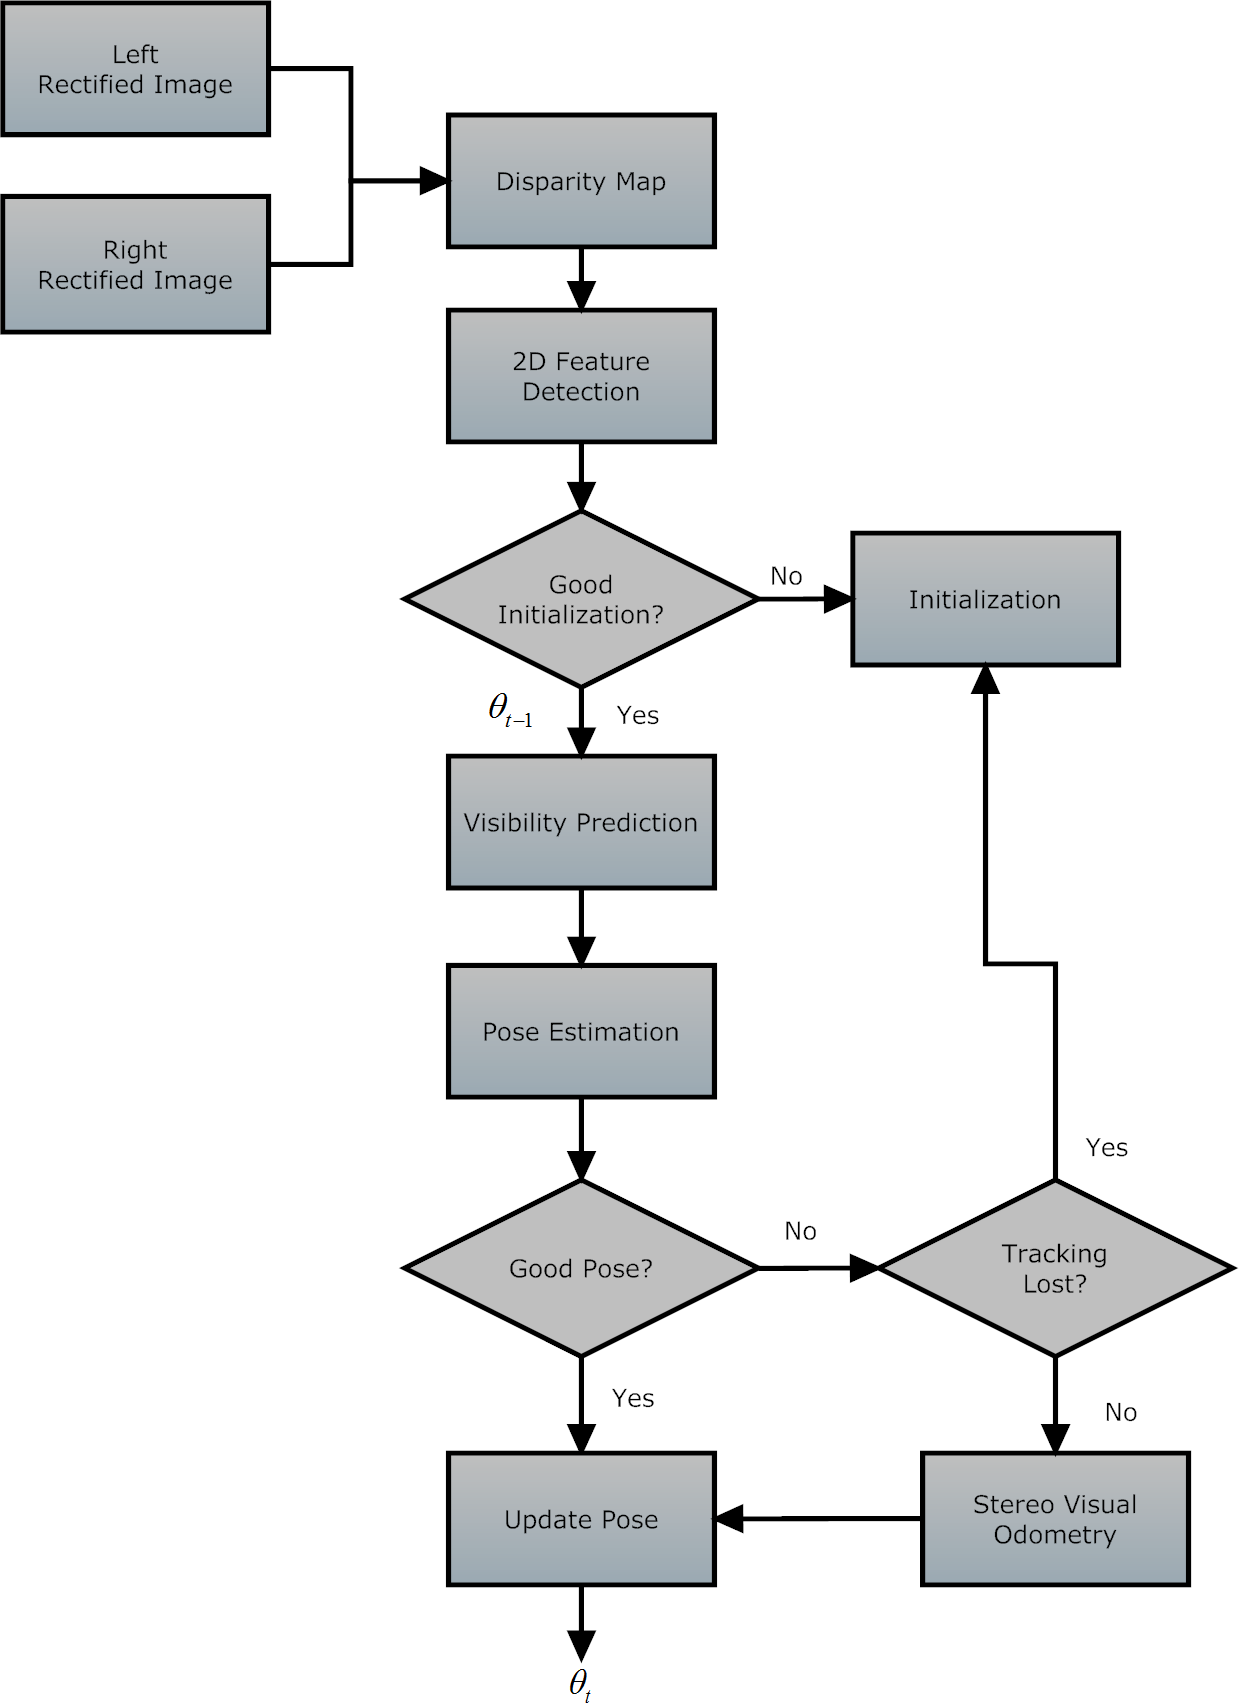
\includegraphics[width=\linewidth]{images/vision_based_localization.png}
  \end{center}
  \caption{Overall overview of our vision-based localization framework with visibility prediction.\label{fig:vision_localization}}
\end{figure}
%
\PFA{If we run out of space, we can skip this figure}
